\documentclass[conference]{IEEEtran} % or another class, depending on your target conference

% Packages
\usepackage{graphicx} % For including images
\usepackage{amsmath}  % For mathematical formulas
\usepackage{hyperref} % For hyperlinks
\usepackage{cite}     % For handling citations
\usepackage{caption}  % For customizing captions
\usepackage{float}
\usepackage{wrapfig}


% Title
\title{Multi-Step Object Re-Identification on Edge Devices: A Pipeline for Vehicle Re-Identification}

% Author(s)
\author{
	\IEEEauthorblockN{Tomass Zutis, Anzelika Bureka, Janis Judvaitis, Janis Arents, Modris Greitans, Peteris Racinskis}
	\IEEEauthorblockA{
		Institute of Electronics and Computer Science, Latvia\\
		janis.arents@edi.lv
	}
}

% Document
\begin{document}
	
	% Title page
	\maketitle
	
	% Abstract
	\begin{abstract}
A method that leverages a multi-step process focused on extracting and using object features for object re-identification is described. The proposed pipeline includes steps such as: detecting an object, converting its features into a vector embedding, storing this embedding in a vector database, and then querying the database to find the same or similar objects based on their feature embeddings. This approach allows for the identification of the same object across different images or cameras, even in varying locations, such as in Vehicle Re-Identification scenarios. For situations where re-identification needs to happen in outdoor environments or on-the-go, implementing this process on edge devices becomes crucial. Therefore, multiple ways to tailor the pipeline and its outputs for edge devices are outlined and investigated. The presentation provides a detailed explanation of the pipeline’s structure and how it functions on edge devices, along with the experimental setup demonstrating its application, particularly in vehicle re-identification.
	\end{abstract}
	
	% Keywords
	\begin{IEEEkeywords}
		Re-Identification, Feature extractions, Vector embeddings, Neural networks, Edge devices, Vector 
		databases
	\end{IEEEkeywords}
	
	% Sections
	\section{Introduction}
%	Introduce the problem of vehicle re-identification and the challenges of implementing this on edge devices. Discuss the significance of efficient computation in real-time applications.

Monitoring and recognizing objects in photos and videos has long been a field of interest for many. It has also become a well researched topic ever since computer vision has accelerated it's possibilities, in the last decade especially  \cite{prince2012computer}.
% vajag rakstu par computer vision potential un possibilities, lkm jau vecaaku
 With computer vision came image classification, which helped us classify images based on the object depicted. That gave us the answer to the question: "What is the object in the image?" \cite{lu2007survey}.
 % Te rakstu par object classification
  Later on came great progress in object detection. That could answer the questions of: "Where are the objects in the image?" and "What are the objects in the image". These were great leaps forward if the job was to pay attention to only objects of a specific class and there were multiple of them in a frame. This was first and foremost fostered by the advancement of the Convolutional Neural Network (CNN) and its variants. \cite{du2018understanding}.
  
% Te varetu ieklaut atsauci uz kadu pirmo sasniegumu objektu detektesanaa un pateikt ka vot vini domaja ka tas bija sasniegums
 In this article, however, the authors are looking for a solution that could see these objects of a single class and distinguish between them, using the specific features that exist only for a single individual in a class.
% Te laikam vajag ielikt definiciju no kaada raksta:
 This problem is called object Re-Identification - widely regarded as a sub-problem of image retrieval \cite{li2019object}.In imagery from at least two different cameras, object Re-identification aims to correctly label the same individual after imaging conditions (like scene, lighting conditions, object pose and others) have changed. In fact, this could be repeated for a specific class in any number of scenes, where there are usually more of these class objects visible. These could be images of vehicles, people or even animals or simple in-animate objects that have great intra-class variations (See fig. \ref{fig:fig1}).
 
 We are also in a unique position where there is still a lot of research to be done on re-identification itself, however, at the same time we are faced with the need to tailor these solutions for edge computing to preserve relevance in global technology and research trends. This is because some of the most common applications of re-identification are in traffic and security that use network cameras and cloud computing \cite{barthelemy2019edge} \cite{wang2024efficient}.
 Cities are looking for edge-computing devices using computer vision and deep neural networks to track real-time events in the public space. With the development of the Internet of Everything (IoE), the number of smart devices connected to the internet, the volume of available video footage, and the influx of sensory data have made the large-scale accumulation of big data inevitable \cite{cao2020overview}. This is why fully automated systems are needed to process data and re-identify patterns and objects in the smart cities environment, for no human or group of humans can be employed to process all this data manually and more crucially - in real time.
 
 \begin{figure}[b]
 	\centering
 	\includegraphics[width=0.5\textwidth]{re_id_diagramma_1.png} % Adjust width as needed
 	\caption{There are multiple uses for object re-identification in the smart cities context. Some of them are: people, vehicles, animals and even luggage in transit hubs.}
 	\label{fig:fig1} % Label for referencing the image
 \end{figure}
 
 In the scenario of traffic monitoring, there is the need to re-identify vehicles on the go to: first of all, be able to track them in a road network and, second, model future traffic based on the existing patterns \cite{barthelemy2019edge}. Edge computing proposes a hardware and software solution that would do this in real time - live video feed would be received from a network camera, that's deployed in the area of interest and the video analytics (i.e. detection and re-identification algorithms) are run directly on the edge device and only the results of the processing are transmitted.
 
 The natural solution to the object re-identification problem in these circumstances is a pipeline consisting of algorithms designed to cover all the necessary steps for re-identification to work. We argue that constructing a pipeline that receives live video feed, processes the frames to extract objects from each frame, saves these objects into memory and recognizes the same objects in a different scene's live video feed is possible and we aim to describe it in detail.
 
	
	\section{Related Work and State of the Art}
	
Object re-identification to this day is heavily reliant on extracting robust feature representations for the objects we are trying to save. Differences in lighting, angle, occlusions, multiple models of the same object (vehicle) are an obstacle in getting reliable predictions \cite{kuma2019vehicle}. However, there is more to a working re-identification pipeline than just looking for the best way to produce vector embeddings. We have looked at the state of the art for multiple components of this problem, such ass: Object detection, Object re-identification and feature extractions, Person re-Identification, Vehicle re-identification, Available datasets, Synthetic datasets and Edge implementation.
	
	\subsection{Object detection}
	\label{sec:object detection}
	
		Convolutional neural networks (CNNs) have been incredibly incremental in computer vision tasks, including object detection. YOLO - the "You Only Look Once" model is one of the best performing and regularly maintained choices. The latest YOLO v8 version (in the authors opinion v8 is the latest model with widespread and public support) has shown significant improvements in accuracy and speed \cite{Rath2023online}, which is crucial for real-time applications like ours. YOLO v8 leverages the experience from the previous YOLO versions, having around 10\% better mean average precision in object detection than the previously popular v5 (when comparing medium model size).
	
	\subsection{Object feature extraction}
	
		Feature extraction is used to extract the most distinct features from an image, which is used to describe it. We try to save these features in a low dimensional vector space \cite{salau2019feature}. Before image feature extraction, multiple pre-processing stages are usually employed like normalization, thresholding, binarization, resizing and others. We can expect a model to extract: color, texture, shape, motion and localization features. However, when dealing with one class objects with small intra-class variations specific types of features can be learned by the model like face features in the case of facial recognition.
		
		As of 2024 CNNs have become predominant choices in object features extraction thanks to their strong representation power and the ability to learn deep invariant embeddings \cite{zheng2019joint}.
	
	\subsection{Vehicle re-identification}
	\label{sec:vehicle re-identification}
	
		It is the case that in re-identification, there seems to be a better tailored model for each benchmark out there. For example, in the realm of Vehicle Re-ID benchmarks MBR4B-LAI model by Almeida \textit{et al.} \cite{almeida2023strength} tops the VeRi-776 benchmark, "A strong baseline" model by Huynh \textit{et al.} \cite{huynh2021strong} tops the CityFlow benchmark and the vehiclenet model by Zheng \textit{et al.} \cite{zheng2019vehiclenet} is best at the VeRi benchmark. However we have chosen to pay particular interest to the paper by Zheng \textit{et al.} because of the baseline model that is applicable to all types of object re-identification and feature extraction. In \cite{zheng2017discriminatively} Zheng \textit{et al.} first introduces us to their baseline model and its architecture and demonstrates its capabilities specifically in pedestrian re-identification. In further papers, however, Zheng \textit{et al.} demonstrate tailoring of this baseline to vehicle re-identification \cite{zheng2019vehiclenet}, \cite{zheng2020vehiclenet} and person re-identification \cite{zheng2019joint}. We underline this baseline models usefulness by the versatility of its use in publications, its open code base and customizability and it's entry into most benchmarks. Even though it tops only one of them, it always keeps close to the top in terms of the Rank1 precision, according to the benchmark results on Papers with Code \cite{paperswithcode2024reid}. The model is implemented in Pytorch and is based on ResNet50 pre-trained on ImageNet, although this backbone is customizable.
	
		We will further refer to this model of interest as "baseline model by Zheng \textit{et al.}".
	
	\subsection{Person re-identification}
	
		The goal of Person re-identification is to match a person's visual identity across many different cameras or locations in video or image sequences. The SOTA in person re-identification can also be judged by the benchmark leaderboards available on Papers with code \cite{paperswithcode2024Persreid}. Some of the most important datasets-turned-benchmarks are: the Market-1501, where the current best Rank-1 accuracy is 98.27\% by Sharma \textit{et al.} \cite{sharma2021person}; the DukeMTMC-reID where the current best Rank-1 accuracy is 95.6\% by Wieczorek, \textit{et al.} \cite{wieczorek2021unreasonable}; and the CUHK03 where the current best Rank-1 accuracy is 98.7\% by by Sharma \textit{et al.} \cite{sharma2021person}. A modified version of the baseline model by Zheng \textit{et al.} has made an entry in the CUHK03 leaderboard 6th place in Rank-1 accuracy with 89.63\% and 3rd place in Rank-5 accuracy with 99.01\%.
		
	\subsection{Available datasets}
	\label{sec:available datasets}
	
		One of the most ample vehicle detection datasets - UA-DETRAC comes from Wen \textit{et al.}  \cite{wen2020ua}. The UA-DETRAC benchmark dataset consists of 100 challenging video sequences captured from real-world traffic scenes. It can be used for object detection model training or fine-tuning.
		
		Some of the vehicle or person Re-ID datasets are already previously mentioned in the context of their usage in benchmarks. The VehicleID (PKU VehicleID) dataset has been introduced by Liu \textit{et al.} in \cite{liu2016deep}. It includes 26'267 unique vehicles with 221'763 images in total. Each image is attached with an ID label corresponding to the vehicle identity. It is the dataset with one of the biggest unique ID collections and features pictures with different resolutions and quality of visibility as well as vehicles in motion state. Vehicles are mostly seen, however, from the front and the back only. The VeRi-776 introduced by Xinchen Liu \textit{et al.} in \cite{liu2016deep2} contains 49'357 images of 776 unique vehicles from 20 different cameras. Each image is attached with vehicle ID, bounding box, type, color, brand. The dataset makes up for its smaller set of unique id's compared to the VehicleID with better quality pictures, better visibility and vehicles from all angles not just back and front. The CityFlow dataset introduced by Tang \textit{et al.} in \cite{tang2019cityflow} is part of the AI City challenge and is a traffic camera dataset consisting of more than 3 hours of synchronized HD videos from 40 cameras. The dataset contains 229'680 images and around 700 unique vehicles. The 2020 AI City challenge \cite{aicity2020data} includes this dataset as videos, but also as cropped vehicle images for ReID model training. The quality of images is high and vehicles can be seen from many angles. The difference between this and the previous two widely used datasets is the types of vehicles seen, namely, US American versus Chinese, which creates a great parameter shift (See fig. \ref{fig:fig2}).
	
	 \begin{figure}[t]
		\centering
		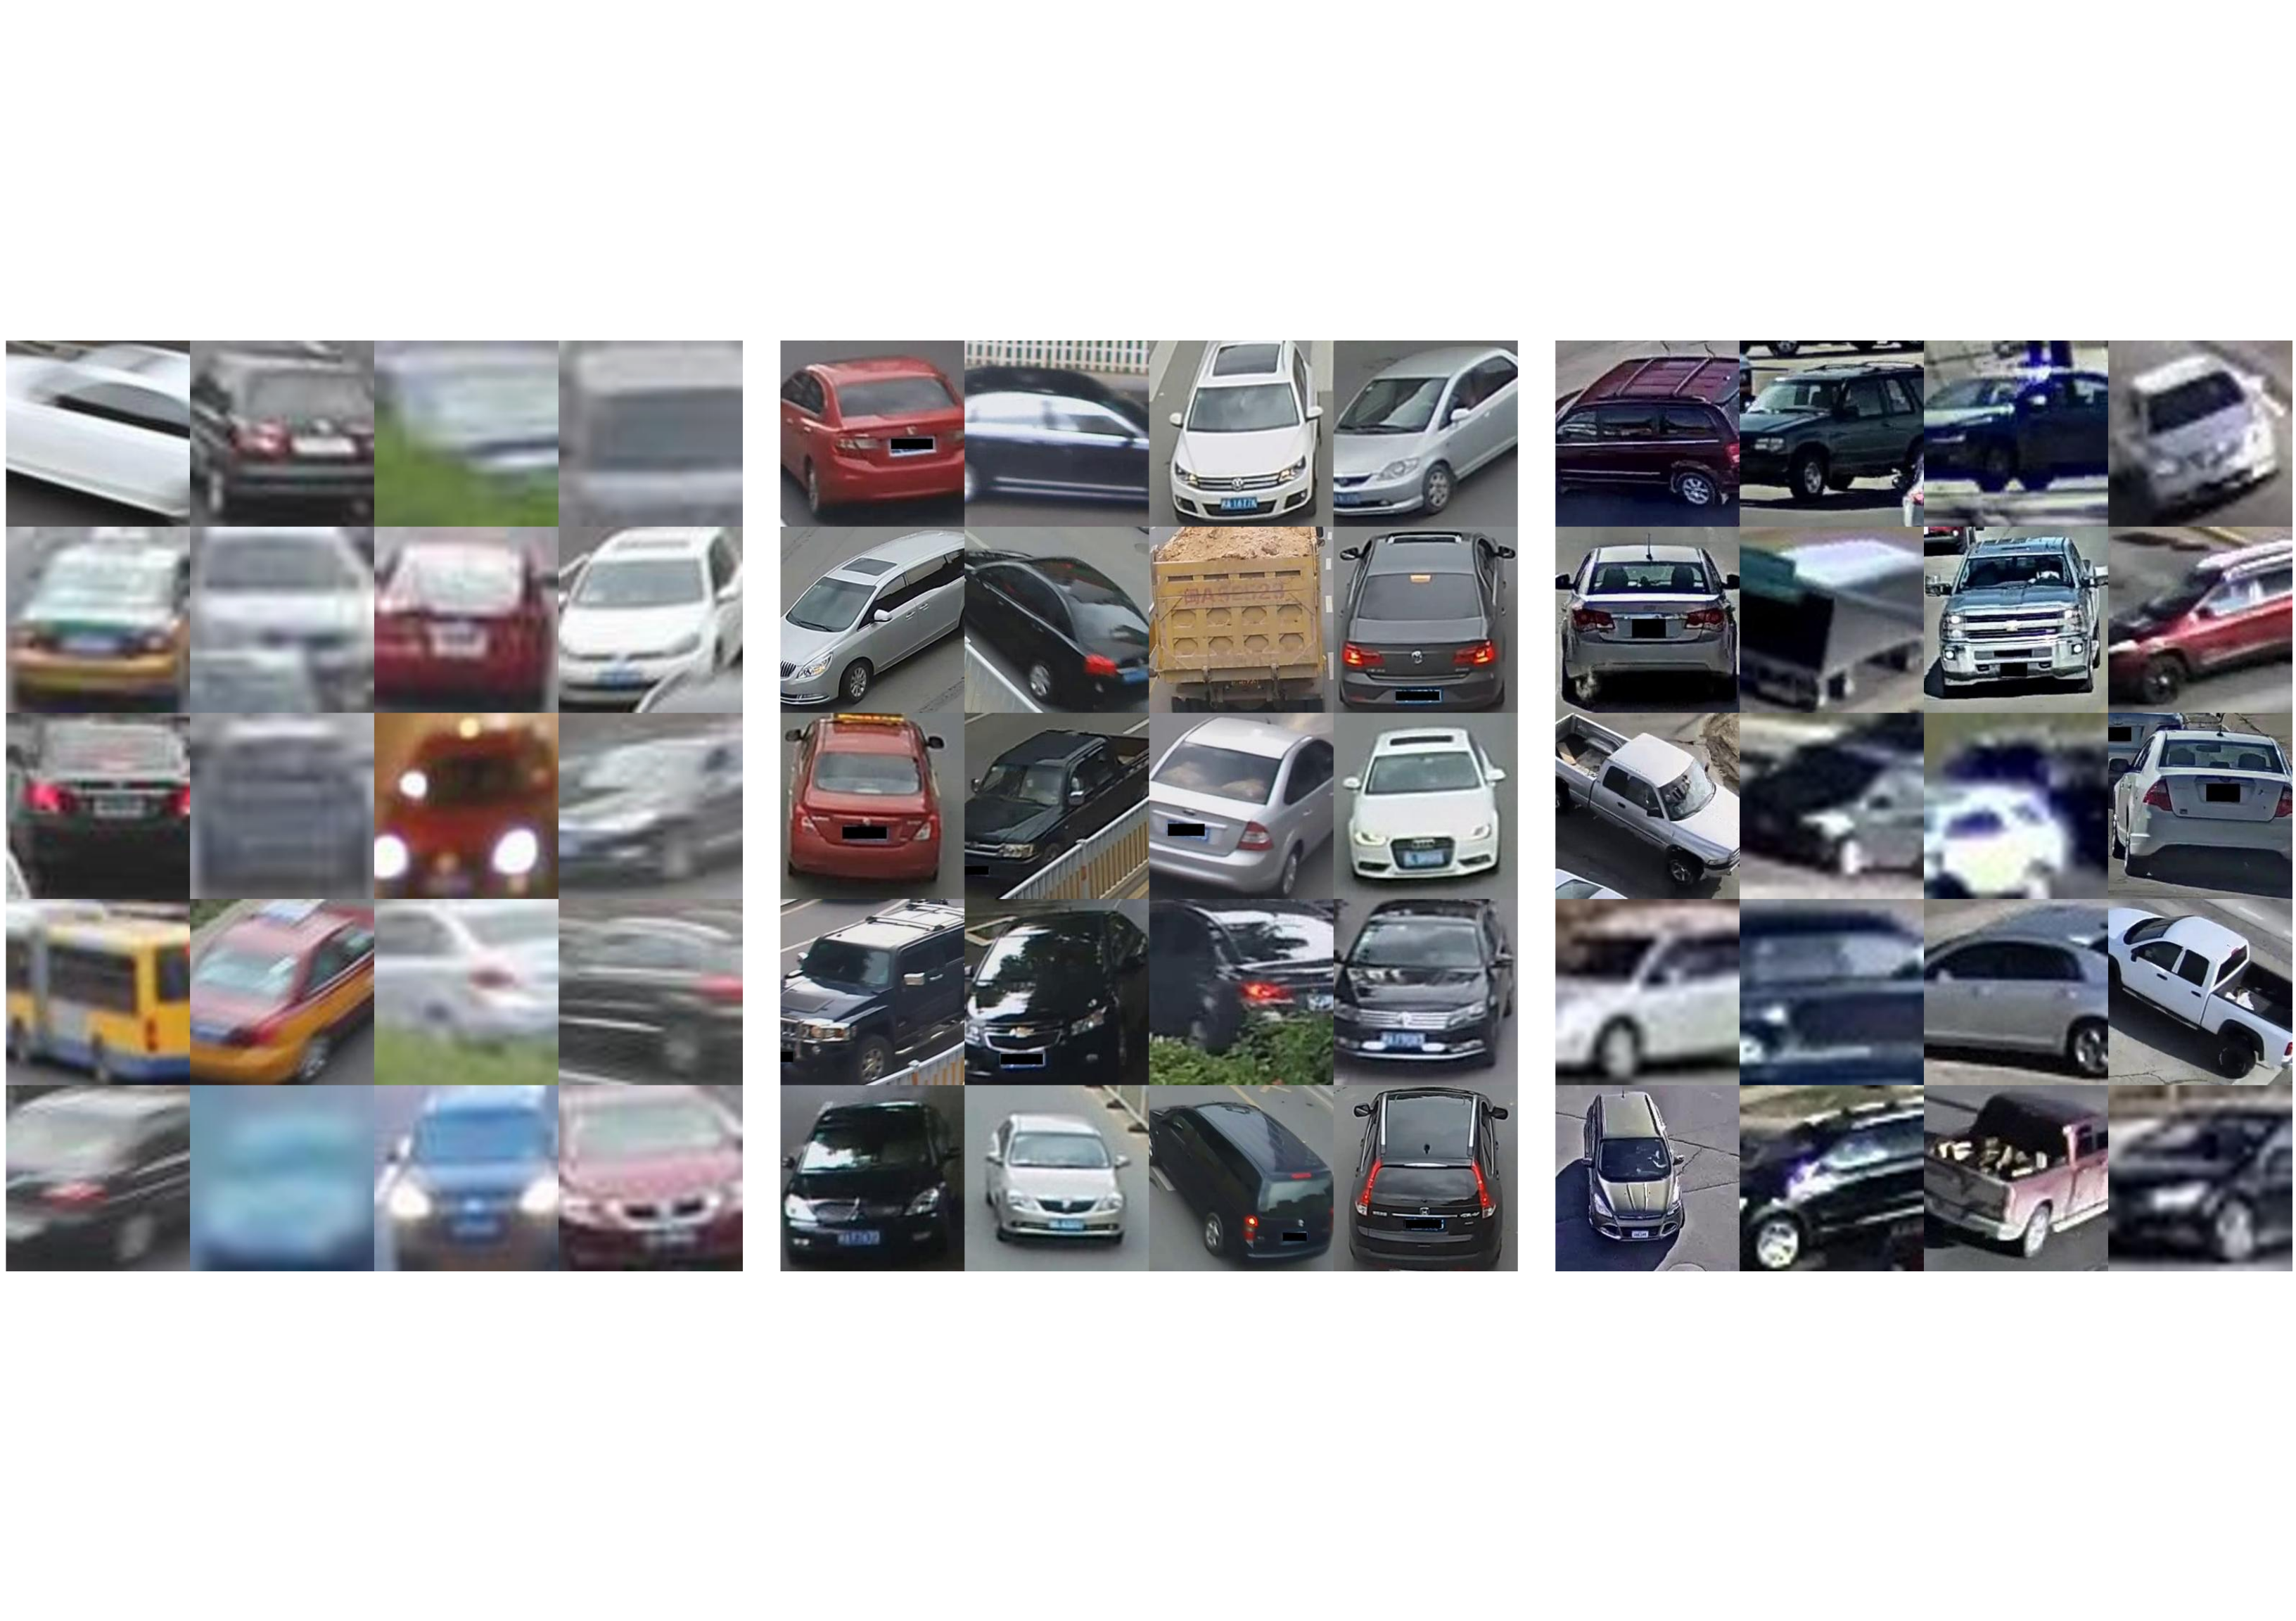
\includegraphics[width=0.5\textwidth]{re_id_diagramma_2.png} % Adjust width as needed
		\caption{The difference between the distribution of vehicles shows us the parameter shift between the (from the left) VehicleID \cite{liu2016deep}, VeRi-776 \cite{liu2016deep2} and CityFlow datasets.}
		\label{fig:fig2} % Label for referencing the image
	\end{figure}
	
	\subsection{Synthetic datasets}
		When creating synthetic standalone datasets, there are risks to learn features that do not generalize to real life images, however, when creating additions to already existing datasets, there is high risk of creating an appendix that has a great parameter shift from the rest of the dataset, thus causing problems with convergence. 
		
		The VehicleX synthetic dataset is created with these problems in mind. It contains generated images with domain adaptation from VehicleID, VeRi-776 and CityFlow datasets \cite{yao2020simulating}. Each of these adapted versions can be paired with the original dataset to enhance learning results.
		
	\subsection{Edge implementation}
		There is a consensus, that if we want to meet the requirements of a real-time system, we need to implement a network that follows the edge-computing paradigm. The edge-computing paradigm means that the video analytics run directly on the device and only the processed results and analytics are transmitted \cite{barthelemy2019edge}. Barthélemy \textit{et al.} have developed a pilot project in Liverpool, Australia, where they use mobility trackers using live CCTV feeds, with twenty sensors deployed over the city with the objective of citywide traffic monitoring in real-time. The devices had the ability to transmit the outputs either over Ethernet or LoRaWAN networks and had two main components: 1.) an NVIDIA Jetson TX2 high performance and power efficient embedded computing device with special units for accelerating neural network computations used for image processing and running Ubuntu 16.04 LTS and 2.) a Pycom LoPy 4 module handling the LoRaWAN communications.
		 
	
	
	
	
\section{Proposed Methodology}
	
	In this chapter we would like to describe the proposed sequence of processes that would enable object re-identification: Object detection, feature extraction and saving and querying for an object in a vector database. We will touch on how these components fit together and how each part could be improved to better serve the common outcome. We will also introduce the application of this methodology in a smart city environment - the Vehicle ReID pipeline.
	
	\subsection{Object detection}
	
		In a scenario, where we are served with images or video frames that have objects of interest included, but not necessarily have these images cropped to the dimensions of the object, we need to find the objects in the image and decide on the extent of their size. This is possible by employing an object detection algorithm.
		 
		In theory, one could train or fine-tune their own object detection model to tailor for a specific object class. However, the latest off the shelf detection models are able to detect vehicles or people, for example, with very high precision. As mentioned in the \ref{sec:object detection} section YOLO v8 model is regarded as very accurate and suitable for real-time applications.
		 
		We will be using the YOLO v8 model to detect the objects of a specific class, determine their bounding boxes and saving cropped out images of these object bounds.
	
	\subsection{Feature extraction}
	
		Once we have cropped images of the objects, we need to extract their features and turn them into vector embeddings. This can be done with a re-identification model, that has learned to extract the features of specific objects and save them in an embedding. For this we will use the baseline model by Zheng \textit{et al.} As described in \ref{sec:vehicle re-identification} section, this baseline can be trained to fit vehicle, person or any other object re-identification. The model is implemented in Pytorch and can be readily customized. We will also use the surrounding project code for this model available on \cite{layumiGithub}. The author has provisioned tools to train, finetune, test and visualize the results of the inference process. The model code is available and can be modified in any stage.
		
	\subsection{Saving feature extractions}
		
		Once we have managed to extract features from such rich data like images, we need to find a way to store and compare the extractions in a computationally inexpensive way. 
		
		These features have been turned into n-dimensional vectors that consist of natural, real or complex numbers, where one number represents a feature or a part of a feature. We should be able to compare these vectors for their similarity, to be able to retrieve the most similar object to the one being queried for. We can do this by using the Cosine similarity function. Cosine similarity is widely used and requires an input of at least two unit-length normalized vector inputs to output a vector distance \cite{bayardo2007scaling}.
		
		Efficient management of vector data would require a Vector database system, so vectors could be stored and queried as efficiently as possible \cite{taipalus2024vector}. This vector database will have to contain vector similarity search complemented by metadata filters. For a very simple interpretation of our task the database entries would simply be in the form of $$ Key:Value = ObjectId:ObjectFeaturesVector $$ while more fields for entries should be easy to add.
		
	\subsection{The Vehicle ReID pipeline}
	
		Having outlined the general components of object re-identification—such as object detection, feature extraction, and storing embeddings—this subsection will introduce the methodology that is specific  to a vehicle re-identification pipeline that is currently under development. This allows the paper to take on a more practical meaning and tests these ideas in real-life.
		
		We propose a pipeline that would take in video frames from a network camera \textit{x}, detect the vehicles in the frames, crop images of the vehicles and save them, turn these cropped images into feature embeddings and then save them in a vector database. The same process would be repeated for a different camera \textit{y ... z}, so that vehicles could be re-identified from camera \textit{x} to \textit{y ... z} or vice versa (see fig. \ref{fig:fig3}).
		%\clearpage
		\begin{figure*}[h]
			\centering
			\includegraphics[width=\textwidth]{re_id_diagramma_3.png} % Adjust width as needed
			\caption{The proposed structure of the re-identification pipeline.}
			\label{fig:fig3} % Label for referencing the image
		\end{figure*}
		
		To make sure we are developing a functional pipeline and are able to monitor the performance of each step we need to split the process into two parts, at least during the development stage:
		
		\begin{itemize}
			\item \textbf{Vehicle counting and tracking}
			
			 The purpose of this process will be to count, track and save information about the vehicles that have passed through the view of a single camera. It should receive the videos from a network camera, detect the vehicles, start tracking them and establish the sectors where we count incoming and outgoing cars (for example entries and exits in an intersection). The count, entry and exit times of cars should be continuously logged.
			\item \textbf{Vehicle Re-Identification}
			
			 Once we have vehicles detected and tracked, we need to decide on an approach about where and how often images of vehicles should be cropped out of the frame. Then we need to save these images, create feature extractions and save them in a vector database.
		\end{itemize}
	
		We will also need to make sure that the methods that make up the pipeline are well tailored for our purpose. We introduce the following points of action:
		\begin{itemize}
			\item \textbf{Establishing sensible counting and tracking solutions}

			We need to develop a solution that counts and tracks vehicles reliably, so that we know that the ReID process after that can run smoothly. We also need to keep a reliable log for supplementing the accuracy of ReID and analysis of the traffic flow.
			
			\item \textbf{Finding the best approach to save images of vehicles}

			It might be important to figure out where and how often should vehicles be cropped out of the frame. A specific position in the camera-view might be more advantageous to save the vehicle and could produce a better feature vector. Complimentary to that, saving the vehicle in multiple positions in the same view might make it more recognizable in a different camera.
			
			\item \textbf{Training the ReID model on different datasets}
			
			We need to make sure, that we have tried all of the most widely used and publicized datasets (mentioned in \ref{sec:available datasets}), to see which fits best for our pipeline.
			
			\item \textbf{Using ensemble modeling}

			An approach with including multiple models in feature extraction should be investigated, in case a single model can not deliver a high accuracy.
			
			\item \textbf{Going over model hyper-parameters}
			
			We need to go over many hyper-parameters during model training. It is valuable to make sure that the default training parameters listed for the baseline model by Zheng \textit{et al.} also fits best for our use case.
			
			\item \textbf{Experimenting with changing the baseline model architecture}

			It can be valuable to see if changes in the architecture or prediction head of the baseline model by Zheng \textit{et al.} could improve accuracy.
			
		\end{itemize}
	
				
		% Te mes iepazistinam sikak ar niansem ka piemeram network camera un to, kaa trennesim modeli konkreti ar vehicle datasetiem utt.
		\subsection{Testing the proposed methodology}
			Since the pipeline is in development, we will first need to conduct a series of tests for individual components and use cases, before we can bring the whole pipeline together for testing.
			
		\begin{itemize}
			\item \textbf{Testing on a dataset}
			
			We need to test the model itself on a dataset to see the accuracy with which the model makes predictions in a very controlled environment such as cropped pictures of vehicles. However, this does not mean that the model has to be tested exclusively on test data of the same dataset, we could also test the model on vehicle images from the network cameras we plan to be using it on.
			
			\item \textbf{Testing on video scenarios}
			
			To test all the components of the re-identification process part of the pipeline we might choose a pre-recorded scene of traffic that has ground truth available. We could skip the object detection and tracking part, hence the ground truth would let the pipeline know where the cars in the frame are and what is their pre-assigned ID. In this case only the bounding box cropping, feature extraction, saving and querying the database could be tested.
			
			\item \textbf{Creating video scenarios}
			
			We might also choose to record video scenarios and create the ground truth ourselves from the Network cameras available. This way the test will be the closest to the real world scenario we should tailor our pipeline for.\newline
			
		\end{itemize}
		
		Before testing the re-identification functionality, it is important to test the vehicle counting step to make sure the process is accurate. This, however, falls slightly outside of the scope of the paper, so we have purposefully chosen to leave these sections out.
		
		At the end of successful testing of all steps of the pipeline, one should create a video test scenario that starts with object detection and does not count on the ground truth bounding box and pre-assigned vehicle id data, encompassing both: 1.) vehicle counting and tracking and 2.) vehicle re-identification functionalities.
		
		
		
		\subsection{Edge device considerations}
		
		While the pipeline has been tested on a desktop computer with an 8GB GPU, this setup provides a rough estimate of the computational load and performance we might expect on edge devices like the NVIDIA Jetson series \cite{valladares2021performance}. Current work suggests that despite differences in power consumption and architecture, the constraints with desktop testing can offer insights for edge deployment that we wish to implement in the future.

	
	\section{Experimental settings}
		
		While the general steps remain consistent with the proposed methodology, the experimental settings section will detail the practical set-up of mentioned concepts, fitted specifically to the use-cases of vehicle ReID in a smart city setting. We will describe the settings for the Vehicle counting and tracking part of the pipeline, Vehicle Re-Identification part of the pipeline, the available datasets used for training, synthetic data used to augment the datasets, experimenting with ensemble modeling, going over hyper-parameters, experiments with changing the model architecture, creating tests and hardware used.
		
		\subsection{Vehicle counting and tracking}
			In this sub-section we will elaborate on the implementation of the counting and tracking part of the pipeline.
			\subsubsection{Receiving video from a Network camera}
				To simulate a traffic scenario for tracking and ReID applications, we will use 3 AXIS P1427-LE Network cameras \cite{axisCam} that record footage from the same service road and a parking lot.
				We are receiving the video in 1280x960 resolution with $\sim$ 2 fps over RTSP, however, HTTP works as well. A 25-30\% compression rate is employed as well for better data transmission.
				
				The view from the cameras (See fig. \ref{fig:fig4}) can be summarized in the following way:
				
				\begin{figure}[b]
					\centering
					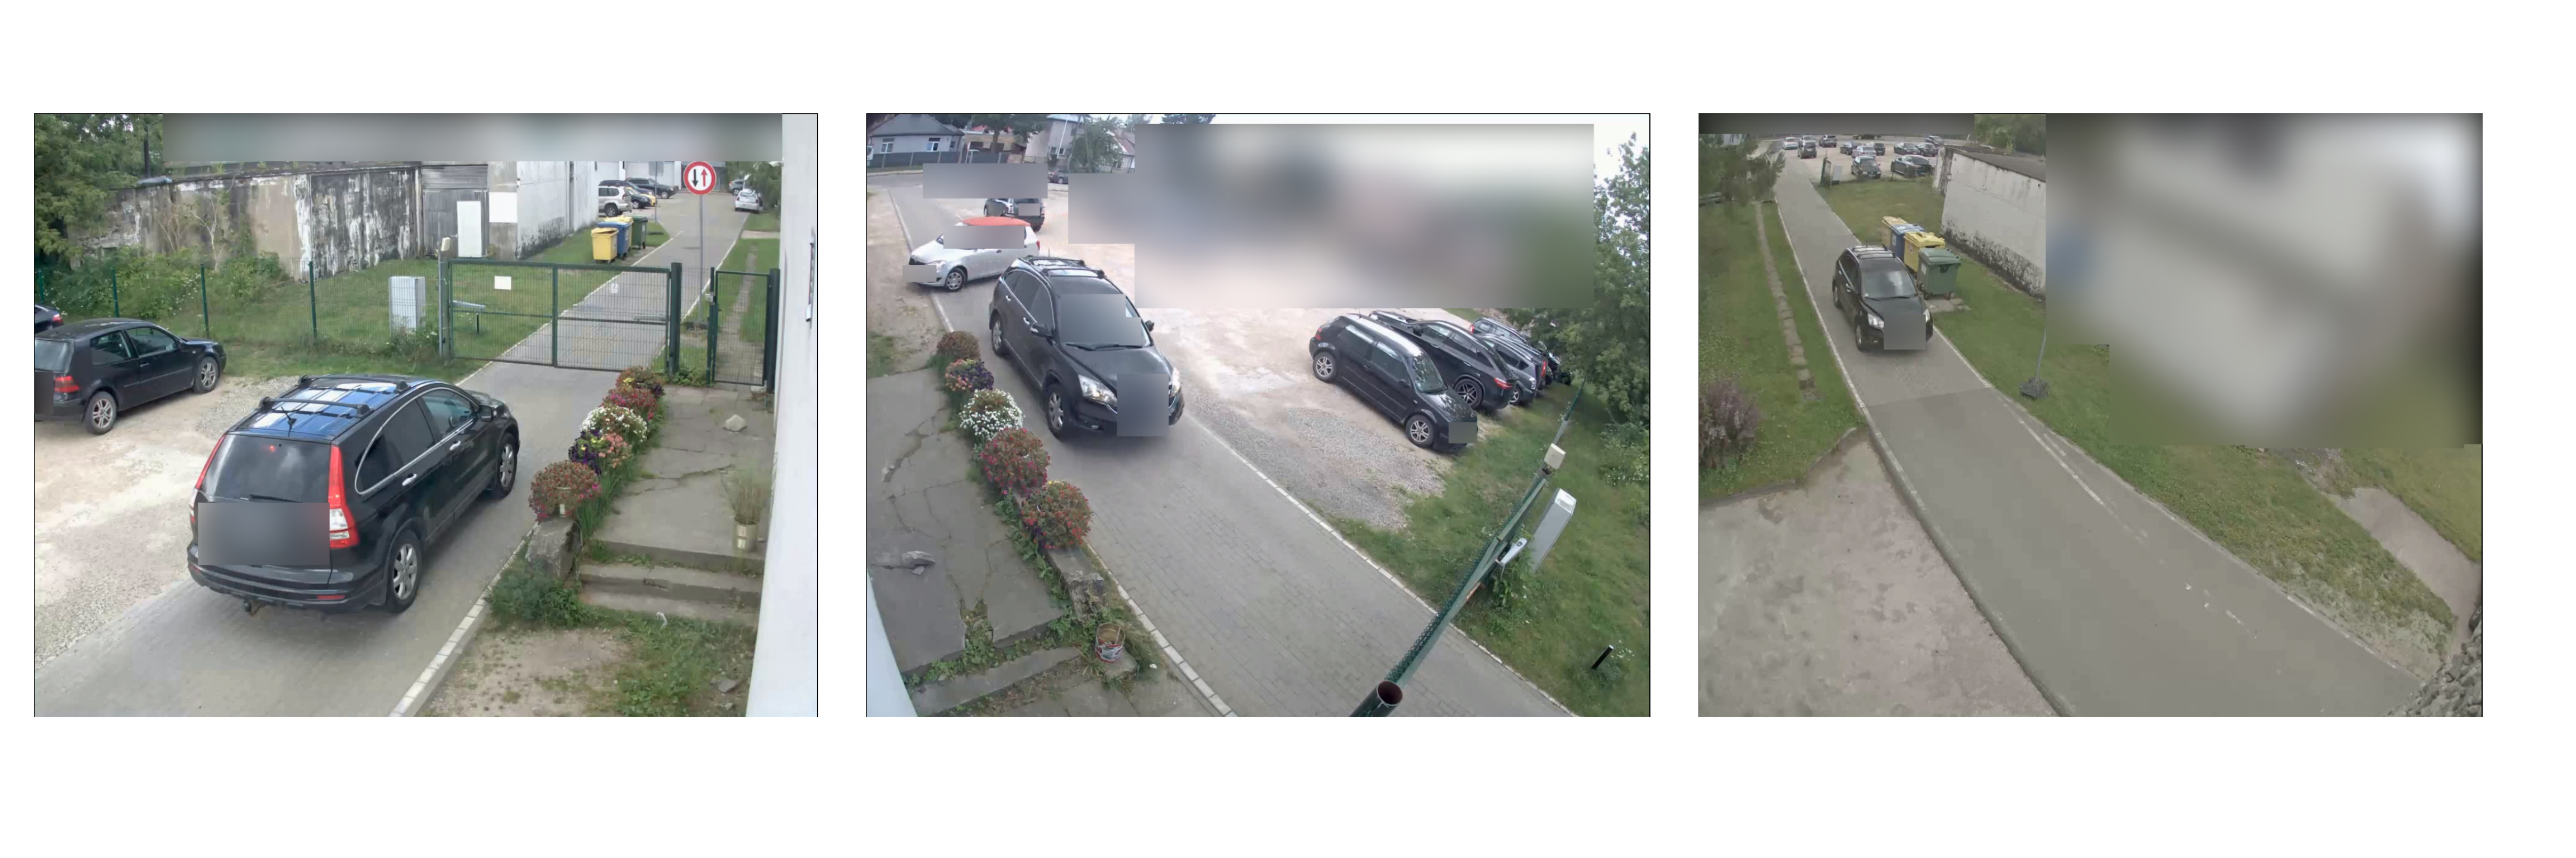
\includegraphics[width=0.5\textwidth]{re_id_diagramma_4.png} % Adjust width as needed
					\caption{The same car visible in cameras (from the left) 1., 2. and 3., respectively.}
					\label{fig:fig4} % Label for referencing the image
				\end{figure}
				
				\begin{itemize}
					\item \textbf{Camera 1.}
					
					This camera sees cars entering and exiting the inner service road from the parking lot from outside of the territory. Gates are also visible. It is located about 3 to 4 meters above ground and generally allows us to see both the front/back of the car and the sides of the car. For non-cargo vehicles, the roof is also visible.
					
					\item \textbf{Camera 2.}
					
					This camera is located above the gates and can see into the parking lot. We can see the opposite side of the car as opposed to camera 1. It is also located about 3 to 4 meters above ground, however, cars are seen more from the front and the back, but skewed sides and roof are visible.
					
					\item \textbf{Camera 3.}

					This camera is located deeper into the territory and generally sees the whole service road with the parking lot in a far distance. The camera is much higher than 1. and 2. and is about 6 to 8 meters above ground. We can see the front/back and roof of the car well, however, the sides are not visible in such quality because of the altitude and angle of the camera.\newline
					
				\end{itemize}
		
	%	Present the experiments, datasets, and evaluation metrics used to validate the method. Include tables, graphs, and illustrations.

	\section{Results}
%	Present the experiments, datasets, and evaluation metrics used to validate the method. Include tables, graphs, and illustrations.
	
	\section{Discussion}
%	Discuss the results and their implications. Highlight the future work on edge device implementation.
	
	\section{Conclusion}
%	Summarize the main findings of the paper and the significance of your work.
	
	% Bibliography
	\bibliographystyle{IEEEtran}
	\bibliography{references} % Make sure you have a .bib file with your references
	
\end{document}
